\section{Mechanical model and dynamics}

\subsection*{Q1: Spring constant from a stationary analysis}

A \SI{1}{\micro\newton} test force is applied to the mass plate along the
motion axis and the spring constant follows from $k=F/u_{y}$.
Table~\ref{tab:q1conv} lists the result for three mesh densities. The value
decreases monotonically with refinement, as expected for displacement-based
finite elements, and changes by only 0.2\% over a factor ten in element
count.

\begin{table}[H]
\centering
\small
\caption{Mesh convergence of the spring constant.}
\label{tab:q1conv}
\begin{tabular}{lcc}
\toprule
mesh & elements & $k$ (\si{\newton\per\meter})\\
\midrule
coarse & 4\,516  & 36.99\\
normal & 12\,709 & 36.87\\
fine   & 44\,563 & 36.79\\
\bottomrule
\end{tabular}
\end{table}

The FEM gives $k=\SI{36.8}{\newton\per\meter}$, 8.7\% below the Part~1
estimate of \SI{40.30}{\newton\per\meter} from four fixed-guided beams,
\begin{equation}
  k_{\mathrm{P1}} = \frac{4E_{Si}\,t\,W_{b}^{3}}{L_{b}^{3}}.
\end{equation}
To find where the 8.7\% comes from, the model was re-solved with the plates
and column made artificially rigid ($E\times1000$ everywhere except the
beams). That returns $k=\SI{39.83}{\newton\per\meter}$, within 1.1\% of the
analytical value. So the discrepancy splits into two parts: about 7.6\% is
compliance of the plates and column, which the analytical model treats as
rigid (the guided beam end rotates slightly when the ``rigid'' body deforms),
and the remaining 1.1\% is shear deformation and 2D continuum effects that
Euler-Bernoulli beam theory leaves out. With $W_{b}/L_{b}=1/15$ the beams
are slender, so a small shear contribution is consistent.

\subsection*{Q2: Eigenfrequency analysis and mode shapes}

Table~\ref{tab:q2modes} lists the first five eigenfrequencies;
Fig.~\ref{fig:modes} shows the modal displacement maps. The fundamental mode
at \SI{496.3}{\kilo\hertz} is the actuation mode: the shuttle translates
along $y$ and the four beams take the S-shape of the fixed-guided boundary
condition. Mode 2 is an in-plane rocking of the shuttle. Modes 3-5 sit
within \SI{4}{\kilo\hertz} of each other and belong to the comb fingers: 20
nearly identical \SI{20}{\micro\meter} cantilevers form a band of
collective bending modes. A single-finger estimate,
$f=0.56\,(W_{c}/L_{c}^{2})\sqrt{E/\rho}\approx\SI{3.4}{\mega\hertz}$, lands
on the band. Frequencies changed by less than 0.1\% between the normal and
fine mesh.

\begin{table}[H]
\centering
\small
\caption{First five eigenfrequencies (fine mesh).}
\label{tab:q2modes}
\begin{tabular}{clc}
\toprule
mode & character & $f$ (\si{\kilo\hertz})\\
\midrule
1 & shuttle translation along $y$ (actuation mode) & 496.26\\
2 & in-plane rocking of the shuttle                & 2\,542.7\\
3 & finger band, collective in-phase bending        & 3\,308.1\\
4 & finger band, alternating pattern                & 3\,311.2\\
5 & finger band, higher spatial pattern             & 3\,311.2\\
\bottomrule
\end{tabular}
\end{table}

Part~1 predicted $f_{0}=\SI{661.9}{\kilo\hertz}$, 33\% above the FEM value.
The ratio is fully accounted for by the stiffness and mass corrections:
\begin{equation}
  \frac{f_{\mathrm{FEM}}}{f_{\mathrm{P1}}}
  = \sqrt{\frac{k_{\mathrm{FEM}}}{k_{\mathrm{P1}}}\cdot\frac{m_{\mathrm{P1}}}{\meff}}
  = \sqrt{0.913\times0.613} = 0.748
  \quad\Rightarrow\quad \SI{495}{\kilo\hertz}.
\end{equation}
Here $\meff = k/(2\pi f_{1})^{2} = \SI{3.79}{\pico\gram}$: the figure-true
shuttle mass of \SI{3.54}{\pico\gram} plus about 36\% of the beam mass, close
to the textbook fraction for a distributed fixed-guided beam.

One limitation should be stated. A 2D in-plane model cannot show
out-of-plane modes. The out-of-plane bending stiffness of the beams is
$(t/W_{b})^{2}=1/625$ of the in-plane one, so the physical device has an
out-of-plane mode near \SI{20}{\kilo\hertz}, far below all modes in
Table~\ref{tab:q2modes}. The assignment asks for the 2D model, so this mode
is outside the scope here, but a 3D design check would have to start with it.

\begin{figure}[H]
\centering
\begin{subfigure}{0.49\textwidth}
  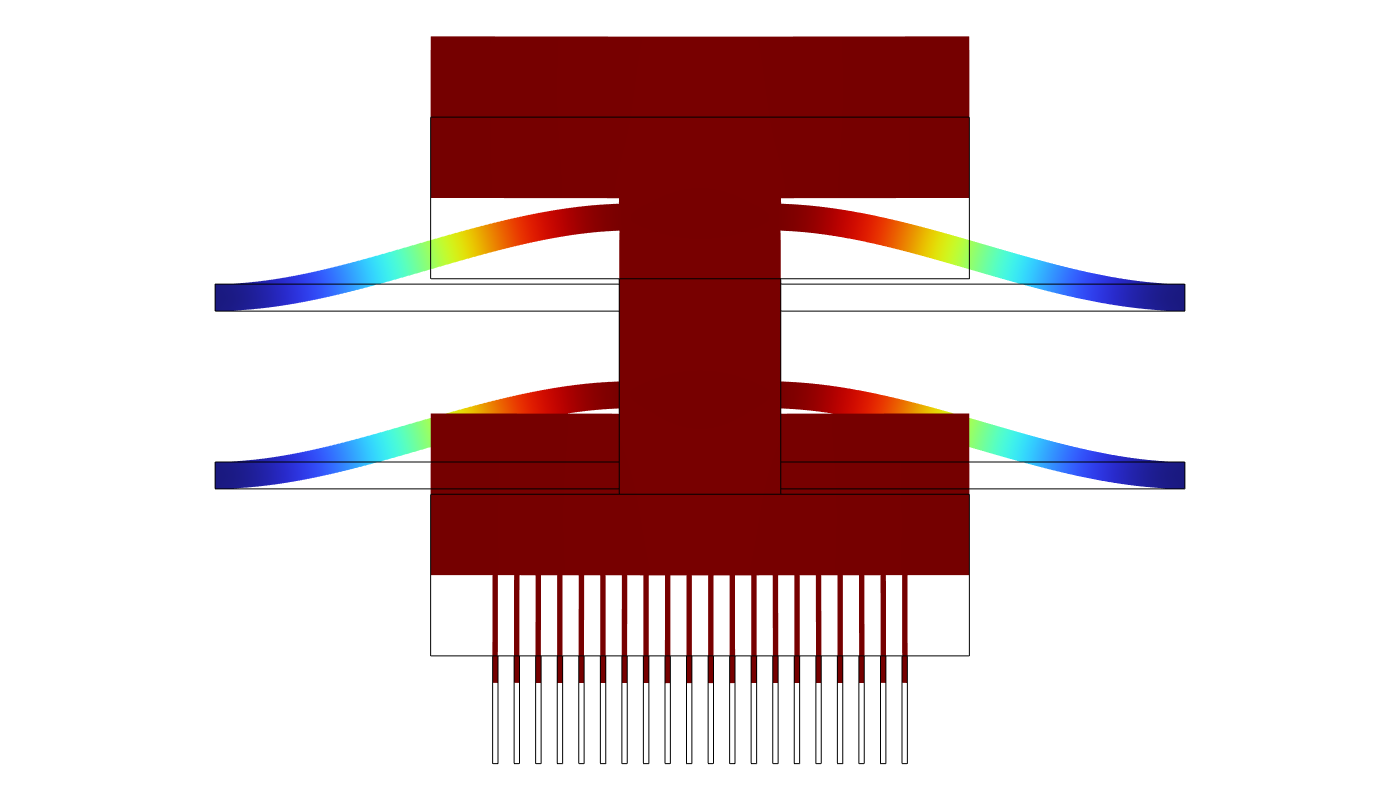
\includegraphics[width=\linewidth]{figures/q2_mode1_496kHz.png}
  \caption{Mode 1, \SI{496}{\kilo\hertz}.}
\end{subfigure}
\hfill
\begin{subfigure}{0.49\textwidth}
  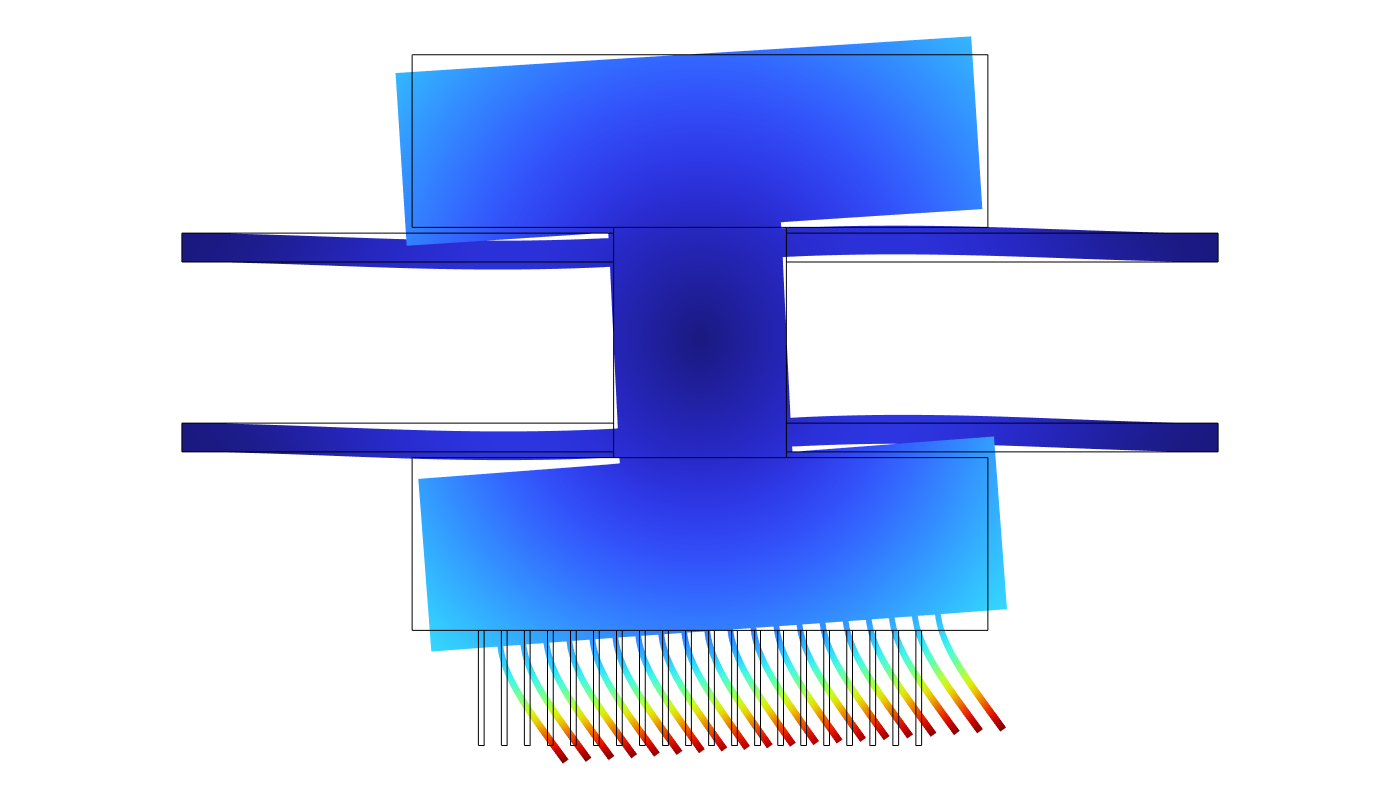
\includegraphics[width=\linewidth]{figures/q2_mode2_2543kHz.png}
  \caption{Mode 2, \SI{2543}{\kilo\hertz}.}
\end{subfigure}\\[4pt]
\begin{subfigure}{0.32\textwidth}
  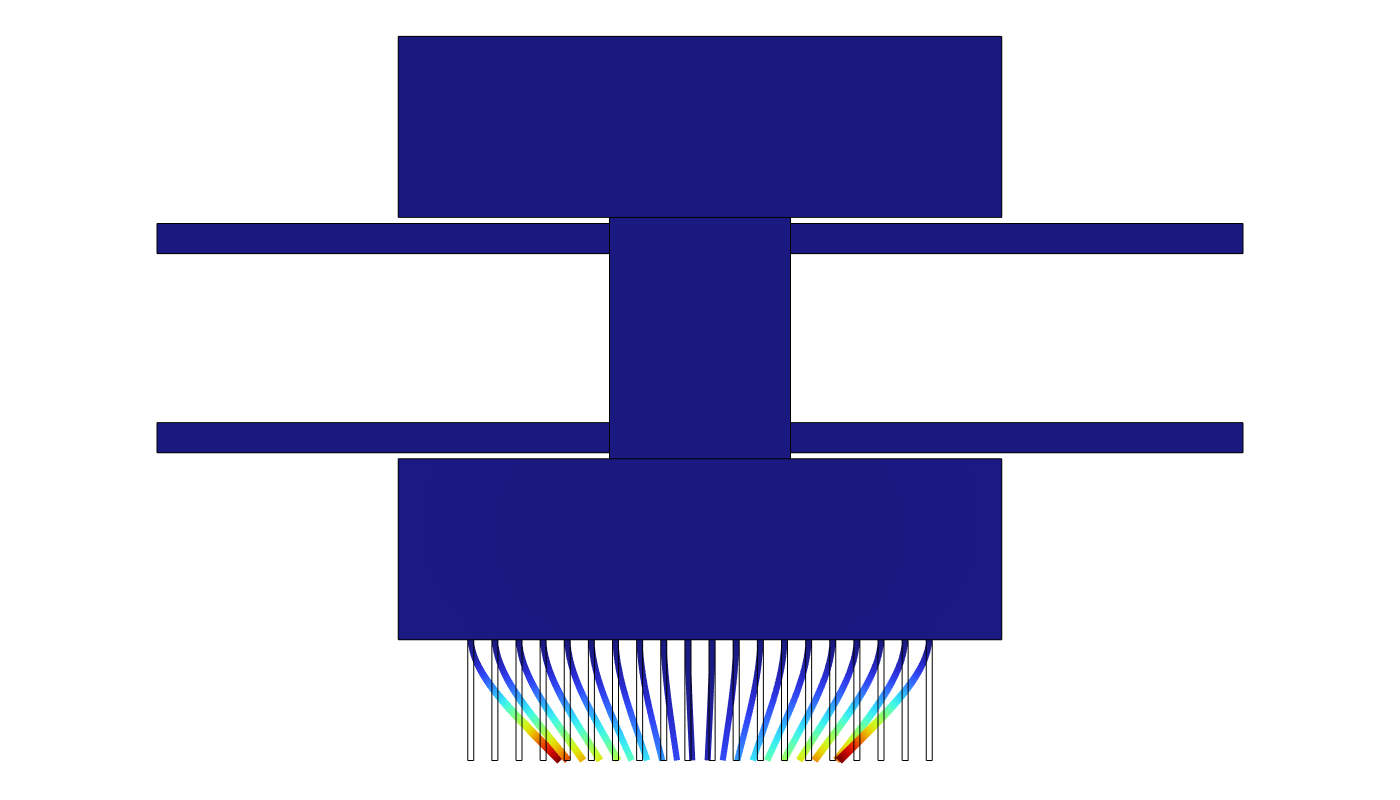
\includegraphics[width=\linewidth]{figures/q2_mode3_3308kHz.png}
  \caption{Mode 3, \SI{3308}{\kilo\hertz}.}
\end{subfigure}
\hfill
\begin{subfigure}{0.32\textwidth}
  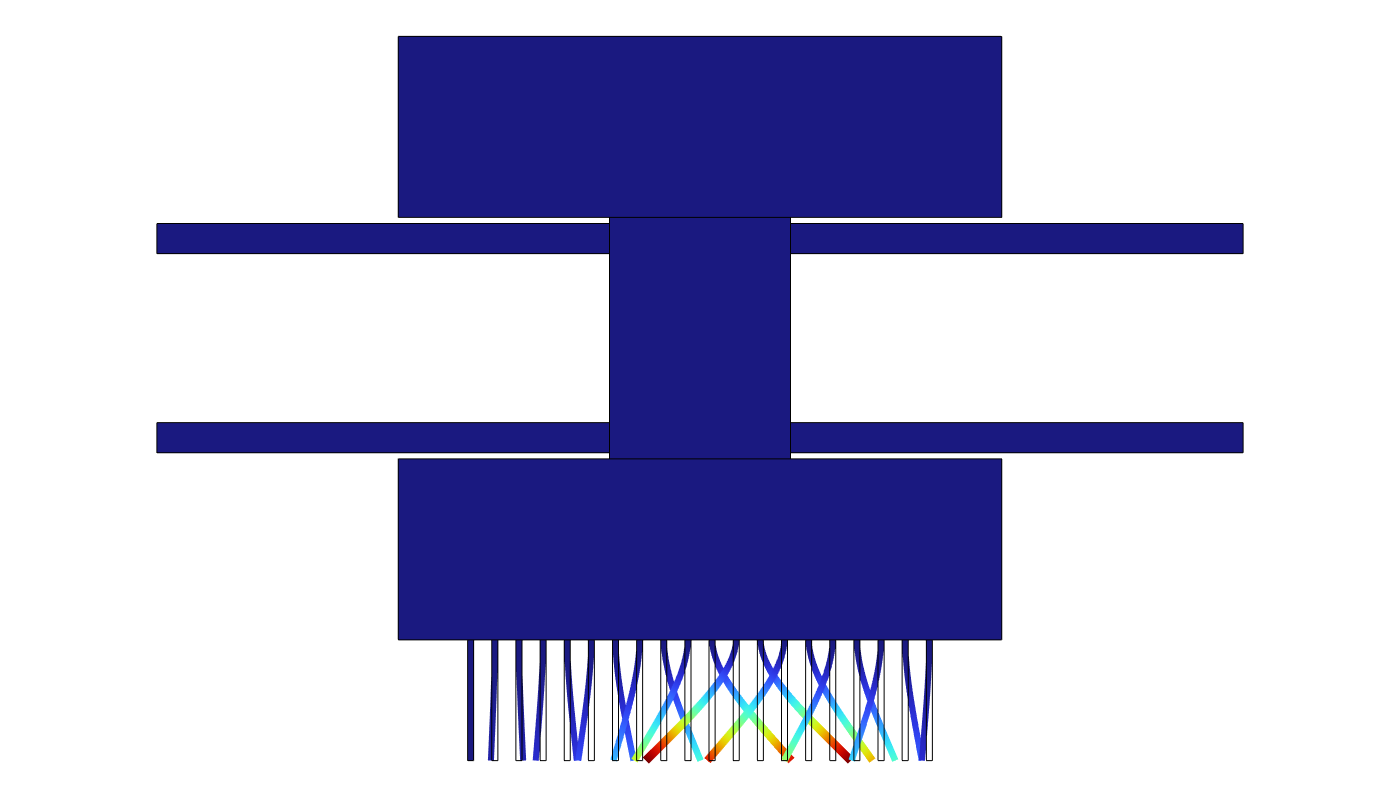
\includegraphics[width=\linewidth]{figures/q2_mode4_3311kHz.png}
  \caption{Mode 4, \SI{3311}{\kilo\hertz}.}
\end{subfigure}
\hfill
\begin{subfigure}{0.32\textwidth}
  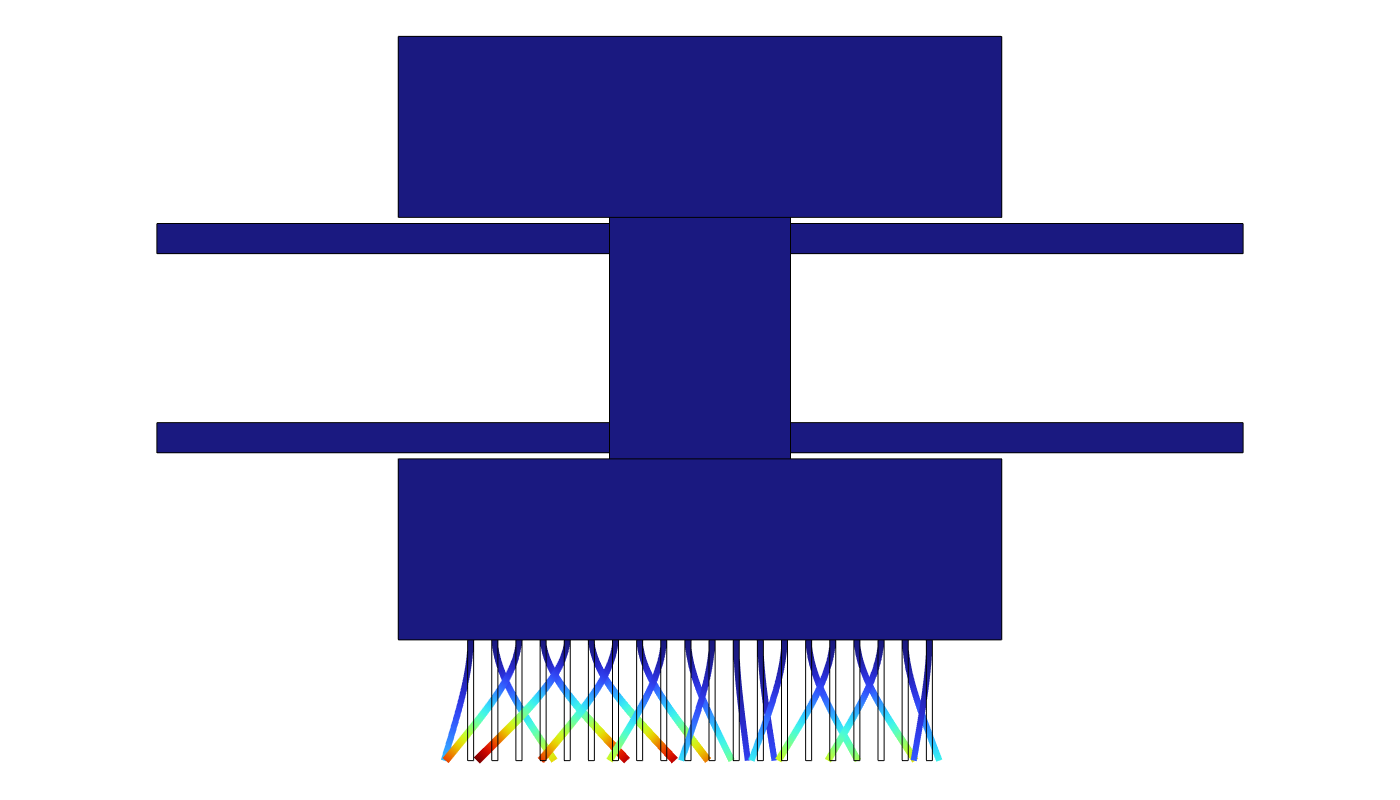
\includegraphics[width=\linewidth]{figures/q2_mode5_3311kHz.png}
  \caption{Mode 5, \SI{3311}{\kilo\hertz}.}
\end{subfigure}
\caption{Modal displacement maps of the first five modes (colour: total
displacement, normalised per mode). Mode 1 is the actuation mode; modes 3-5
are collective comb-finger modes.}
\label{fig:modes}
\end{figure}

\subsection*{Q3: Rayleigh damping and force-step response}

The assignment asks for $Q=83$. Rayleigh damping gives a modal damping ratio
\begin{equation}
  \zeta(f) = \frac{\alpha_{dM}}{4\pi f} + \beta_{dK}\,\pi f ,
\end{equation}
with two free parameters but only one target, $\zeta(f_{1})=1/(2Q)$. I chose
pure stiffness damping, $\alpha_{dM}=0$ and
\begin{equation}
  \beta_{dK}=\frac{1}{2\pi f_{1} Q}
            =\frac{1}{2\pi\cdot\SI{496.26}{\kilo\hertz}\cdot 83}
            =\SI{3.87e-9}{\second},
\end{equation}
because $\beta$-damping grows with frequency and therefore also suppresses
the \SI{3.3}{\mega\hertz} finger band; mass-proportional damping would have
left those modes nearly undamped on top of the response.

The transient applies a \SI{1}{\micro\newton} step to the mass at $t=0$ and
runs to \SI{400}{\micro\second} with a relative tolerance of $10^{-5}$.
Figure~\ref{fig:q3step} shows the result. The response rings at $f_{1}$,
overshoots to $1.96\times$ the static value (the ideal underdamped limit is
2), and decays inside the analytic envelope $e^{-\zeta\omega_{1}t}$. The
final value of \SI{27.11}{\nano\meter} matches $F/k=\SI{27.12}{\nano\meter}$
to 0.05\%.

\begin{figure}[H]
\centering
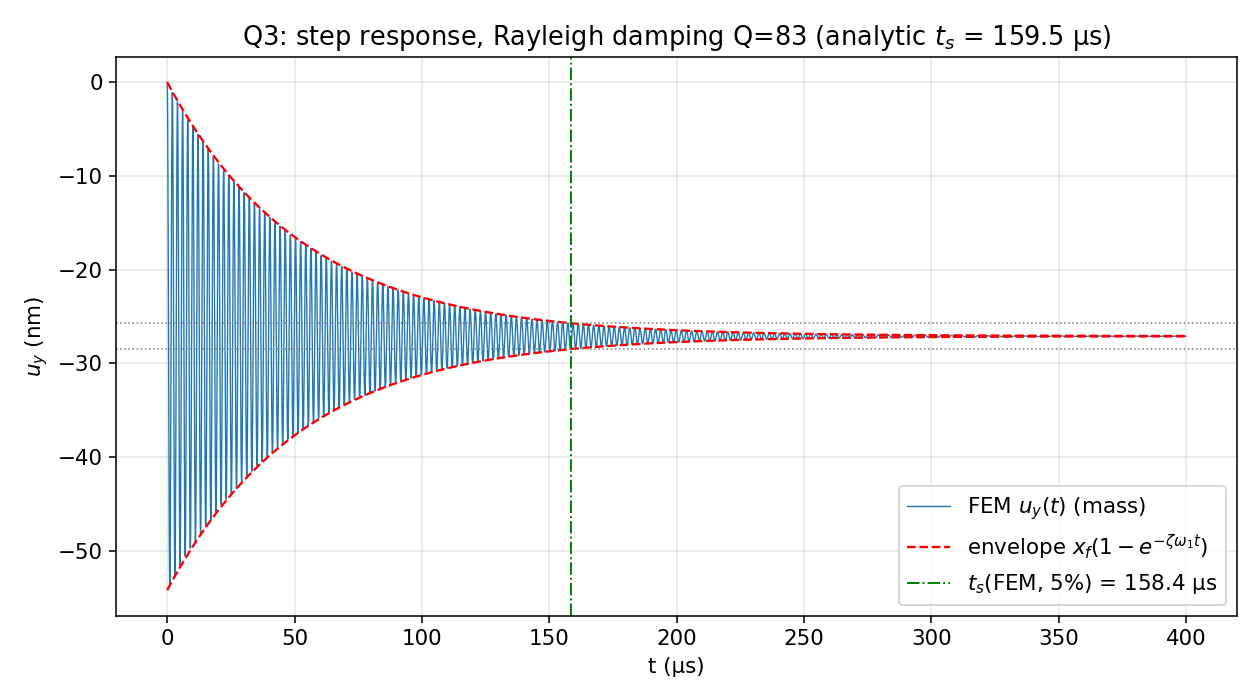
\includegraphics[width=0.85\textwidth]{figures/q3_step_response.png}
\caption{Step response to a \SI{1}{\micro\newton} force with Rayleigh damping
set for $Q=83$. Red dashes: analytic envelope
$x_{f}(1\pm e^{-\zeta\omega_{1}t})$; dotted lines: $\pm5\%$ band; green line:
measured \SI{5}{\percent} settling time.}
\label{fig:q3step}
\end{figure}

The measured $5\%$ settling time is \SI{158.4}{\micro\second}. The analytic
value with the FEM frequency, $t_{s}=\ln(20)/(\zeta\omega_{1})=\SI{159.5}{\micro\second}$,
agrees to 0.7\%, which also confirms that the integrator adds no significant
numerical damping at this tolerance. Part~1 predicted
\SI{139}{\micro\second}. The formula is the same; the inputs differ. Part~1
used its computed $Q=96.8$ where the assignment now fixes $Q=83$, and its
$\omega_{0}$ was 33\% high (Q2). Since $t_{s}\propto Q/\omega$, the two
corrections nearly cancel and the predictions end up closer than the inputs
would suggest.
